\chapter{Analiza wpływu przewagi informacji}
Posiadanie informacji niedostępnej dla pozostałych uczestników rynku bez wątpienia stawia informatora na wygranej pozycji - podczas gdy inni gracze muszą liczyć się z ryzykiem, zysk informatora jest praktycznie pewny. Pozornie oczywista strategia informatora komplikuje się jednak w ujęciu długoterminowym, trzeba wówczas rozważyć problemy pomijalne w kontekście jednorazowego incydentu wykorzystania przewagi informacyjnej. Przede wszystkim, trzeba wziąć pod uwagę, że inni gracze, będąc stratni, mogą zrezygnować z inwestowania na danym rynku lub zmodyfikować swoje strategie w sposób niekorzystny dla informatora. W obu przypadkach informator może długoterminowo stracić stosując najbardziej zyskowną strategię przy założonych stałych strategiach pozostałych graczy. 

Gruntowna weryfikacja optymalnej strategii informatora w zależności od kapitału i liczby obserwujących jest zadaniem kompleksowym - wymaga zdefiniowania alternatywnych do referencyjnej konfiguracji modelu. Rozważamy zatem analizę znacznie prostszą, ale pozwalającą nakreślić wpływ obecności informatora na rynek w zależności od skali jego działania i wskazać potencjalne ograniczenia jego strategii.

\section{Plan symulacji}

Eksperyment rozbijemy na dwa etapy. W pierwszej kolejności nie uwzględnimy obecności obserwujących agentów, skupiając się jedynie na wpływie obecności insidera i jego optymalnych strategiach w zależności od kapitału, jakim dysponuje. Następnie, dla ustalonego kapitału informatora włączymy do symulacji obserwujących agentów i przyjrzymy się, czy dzielenie się informacją jest dla niego korzystne. W obu etapach, dla uproszczenia, przyjmujemy taki sam model obudzeń informatora (generowanych, analogicznie jak w przypadku agentów klasy \textit{ValueAgent}, zgodnie z procesem Poissona zdefiniowanym w tabeli \ref{tab:refconfig}) oraz taki sam scenariusz wyroczni, tzn. przyjmujemy, że w każdym z testowanych przypadków zachodzi zdarzenie $\eta = (t_{\eta}, \Delta_r).$

\subsection{Zależność strategii od kapitału}
Celem strategii informatora jest kupno możliwie najtaniej (sprzedaż możliwie najdrożej) jednostek instrumentu przed oczekiwaną zmianą ceny. Podstawowymi cechami różnicującymi potencjalne strategie informatora są liczba i rozmiar zleceń, w jakich gracz realizuje swoje cele. Spośród zbioru strategii możemy wyróżnić dwie skrajne: dyskretnego informatora, który wykonuje w odstępach czasu szereg zleceń małej lub przeciętnej wielkości, oraz dominatora o praktycznie nieograniczonych środkach, wystawiającego bardzo duże, zauważalne, zlecenia.

Dwie skrajne strategie narzucają zakres planowanych symulacji. Możliwości finansowe informatora definiujemy parametrem \texttt{max\_qty} - maksymalną liczbą jednostek, które może nabyć (sprzedać), zakres ich możliwych wartości wyznaczamy na podstawie rozkładu zleceń. Możliwe rozmiary zleceń informatora \texttt{order\_size} wyznaczamy w oparciu o załączony do konfiguracji referencyjnej rozkład dany tabelą \ref{tab:distmix} - na tej podstawie szacujemy przeciętną oraz przypadki skrajne. 

Dla każdej z rozważanych wartości maksymalnej liczby jednostek \texttt{max\_qty} dobieramy trzy różne wartości \texttt{order\_size} mające odwzorowywać trzy różne realizacje kupna (sprzedaży) \texttt{max\_qty}: w możliwie najmniejszych zleceniach, w kilku partiach oraz w jednym dużym zleceniu. Dokładne wartości parametrów \texttt{max\_qty} i \texttt{order\_size} zostały zawarte w tabeli \ref{tab:simplan1}.
\begin{table}
\caption{Plan symulacji dla konfiguracji zależnych od rozmiaru zlecenia i maksymalnej liczby jednostek } 
\label{tab:simplan1}
% opisać modify, replace, partial cancel, złożenie 
\begin{center}
\begin{tabular}{|p{2cm}|p{2cm}|p{2cm}|}
\hline
\textbf{\texttt{max\_qty}} & \textbf{\texttt{order\_size}} & \textbf{liczba replikacji} \\
\hline 
100 & 5 & 25 \\
 & 25 & 25 \\
 & 100 & 25 \\
\hline
1000 & 25 & 25 \\
 & 250 & 25 \\
 & 1000 & 25 \\
\hline
10000 & 250 & 25 \\
 & 2500 & 25 \\
 & 10000 & 25 \\
\hline
10000000 & 25000 & 25 \\
 & 2500000 & 25 \\
 & 10000000 & 25 \\
\hline
\end{tabular} 
\end{center}
\end{table}
\subsection{Wpływ liczby obserwujących na strategię informatora}
Wartości parametrów \texttt{order\_size} i \texttt{num\_followers} - liczby obserwujących zostały zawarte w tabeli \ref{tab:simplan2}.
\begin{table}
\caption{Plan symulacji dla konfiguracji zależnych od rozmiaru zlecenia i liczby agentów obserwujących informatora} 
\label{tab:simplan2}
% opisać modify, replace, partial cancel, złożenie 
\begin{center}
\begin{tabular}{|p{2cm}|p{2cm}|p{2cm}|p{2cm}|}
\hline
\textbf{\texttt{max\_qty}} & \textbf{\texttt{order\_size}} & \textbf{liczba obserwujących} & \textbf{liczba replikacji} \\
\hline 
10000 & 25 & 10 & 25 \\
& & 50& 25\\
& & 100 & 25\\
& & 500& 25\\
& &1000 & 25\\
\hline
10000 & 100 & 10 & 25 \\
& & 50& 25\\
& & 100 & 25\\
& & 500& 25\\
& &1000 & 25\\
\hline
10000 & 1000 & 10 & 25 \\
& & 50& 25\\
& & 100 & 25\\
& & 500& 25\\
& &1000 & 25\\
\hline

\end{tabular} 
\end{center}
\end{table}



% tabele [liczba replikacji] [kolejne parametry]
%[tutaj opisuję, jakie konfiguracje testowałam w ilu próbach i dlaczego takie]
\section{Analiza wyników}
W pracy omówimy tylko najistotniejsze wnioski wynikłe z analizy wyników symulacji. Całość wyników oraz notatniki podsumowujące całość zebranych danych są załączone jako uzupełnienie pracy oraz udostępnione w \href{https://github.com/AgataCieslik/abides-jpmc-public}{publicznym repozytorium pracy} .
\subsection{Wpływ skali działania informatora na innowację ceny}
Zgodnie z oczekiwaniami, wyniki symulacji wykazują wpływ obecności informatora na kształtowanie się ceny. Przede wszystkim decydujące znaczenie ma tutaj wielkość zaangażowanych środków informatora (wyrażona parametrem \texttt{max\_qty}). Realizacja dużych transakcji znacząco przyspiesza proces uwzględnienia efektu zdarzenia w cenie (Rysunek \ref{fig:meanpriceinn}).
\begin{center}
\begin{figure}
\begin{center}
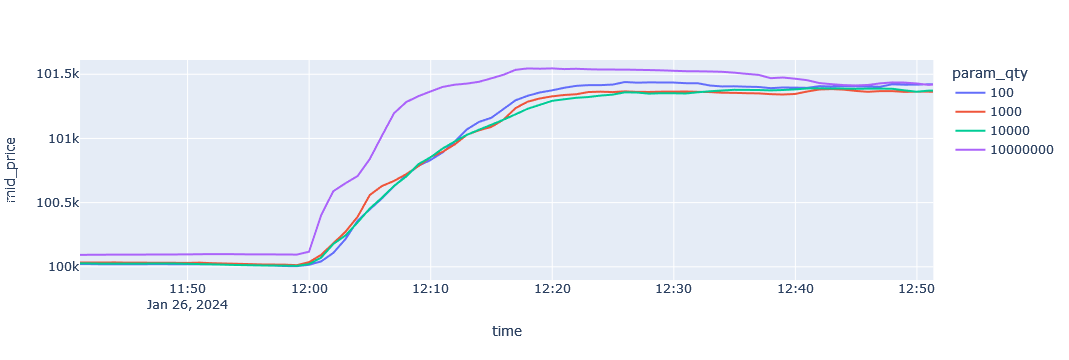
\includegraphics[scale=0.4]{srednia_innowacja_ceny.png}
\end{center}
\caption{Wykres średnich cen w replikacjach pogrupowanych według możliwości finansowania informatora}\label{fig:meanpriceinn}
\end{figure}
\end{center}
Również rozmiar i częstotliwość zleceń wydają się nie pozostawać bez wpływu na proces kształtowania ceny. Sytuację dobrze obrazuje wykres ceny w zależności od parametryzacji dla replikacji (równoważnej realizacji procesu wyroczni) o id 16 (Rysunek \ref{fig:priceinn}).
\begin{center}
\begin{figure}
\begin{center}
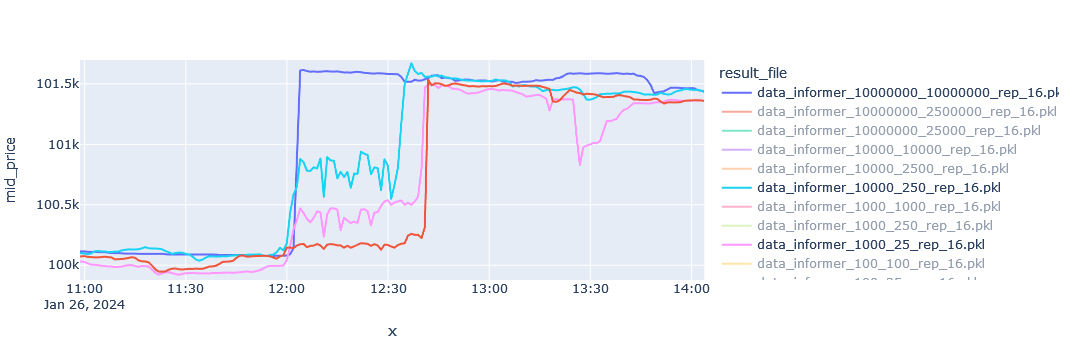
\includegraphics[scale=0.4]{innowacja_ceny.png}
\end{center}
\caption{Wykres ceny w zależności od parametryzacji informatora dla replikacji o id=16}\label{fig:priceinn}
\end{figure}
\end{center}
\subsection{Ograniczenie na maksymalny kapitał informatora} 
Porównując wyniki symulacji w zależności od zaangażowanego kapitału informatora możemy wysnuć hipotezę, że istnieje ograniczenie na maksymalny zaangażowany kapitał gracza z uprzywilejowaną informacją. 
\begin{center}
\begin{figure}
\begin{center}
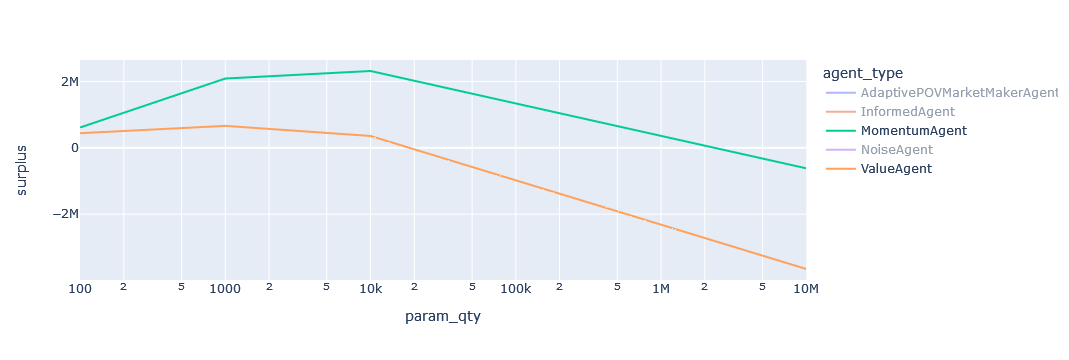
\includegraphics[scale=0.4]{kapital.png}
\end{center}
\caption{Średnie wypłaty agentów klas \textit{ValueAgent} i \textit{MomentumAgent} w zależności od zaangażowanych środków informatora}\label{fig:capital}
\end{figure}
\end{center}
Wnioski opieramy w głównej mierze na analizie wypłat dla graczy konfiguracji referencyjnej \textit{ValueAgent} i \textit{MomentumAgent} (Rysunek \ref{fig:capital}) reprezentujących dwa rzeczywiste nurty inwestowania: strategie oparte na analizie fundamentalnej oraz bazujące na analizie technicznej. Oba typy agentów odnotowują średnio znaczne straty dla maksymalnej wartości środków informatora, co budzi wątpliwości, czy w rzeczywistości zdecydowaliby się realizować do końca swój scenariusz inwestycyjny, równocześnie umożliwiając informatorowi dopełnienie jego strategii zgodnie z planem. 

\subsection{Wpływ strategii informatora na wypłaty innych graczy}
Analiza wyników symulacji wskazała ciekawy konflikt interesów między agentami typów \textit{ValueAgent} oraz \textit{MomentumAgent} - graczom tych typów sprzyjają dwie skrajne strategie informatora (dobrze to widać na przykładzie tabeli wypłat na rys. \ref{fig:gametab}). W przypadku \textit{ValueAgent} najkorzystniejszą strategią informatora jest strategia oparta na zleceniach relatywnie małych rozmiarów, w niewielkim stopniu wpływających na cenę. Z kolei dla agentów typu \textit{MomentumAgent} najkorzystniejsze są strategie wystawiające zlecenia dużych rozmiarów, które wpływają zauważalnie na cenę rynkową i skutkują zaktualizowaniem używanych przez agenta wskaźników analizy technicznej zgodnie z rzeczywistym kierunkiem zmiany ceny w przyszłości. 
\begin{center}
\begin{figure}
\begin{center}
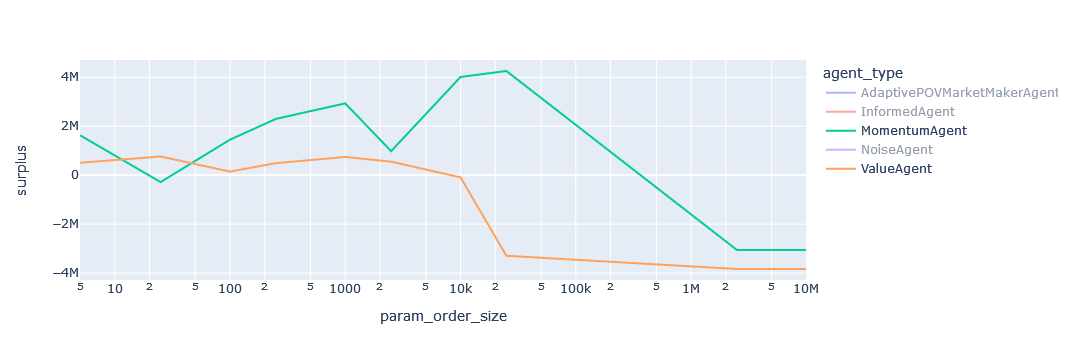
\includegraphics[scale=0.4]{ordersize.png}
\end{center}
\caption{Średnie wypłaty agentów klas \textit{ValueAgent} i \textit{MomentumAgent} w zależności od wielkości zleceń informatora}\label{fig:ordersnum}
\end{figure}
\end{center}
\begin{center}
\begin{figure}
\begin{center}
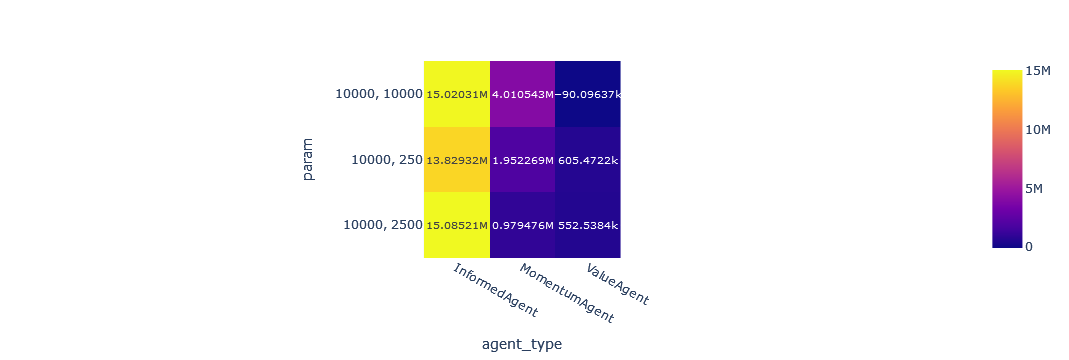
\includegraphics[scale=0.4]{table.png}
\end{center}
\caption{Tabela wypłat graczy dla ustalonego parametru informatora \texttt{max\_qty}=10000}\label{fig:gametab}
\end{figure}
\end{center}
\subsection{Ograniczenie na liczbę obserwujących}
Analiza konfiguracji z włączonymi populacjami agentów - obserwatorów informatora sugeruje, że informator powinien narzucić ograniczenie na rozmiar grupy, której udostępnia rekomendacje. Sporządzone wykresy średnich wypłat (rys.\ref{fig:followers}) zarówno informatora, jak też jego obserwatorów, jasno pokazują, że powyżej 50 agentów w populacji obserwatorów średnie wypłaty obu typów agentów maleją.
\begin{center}
\begin{figure}
\begin{center}
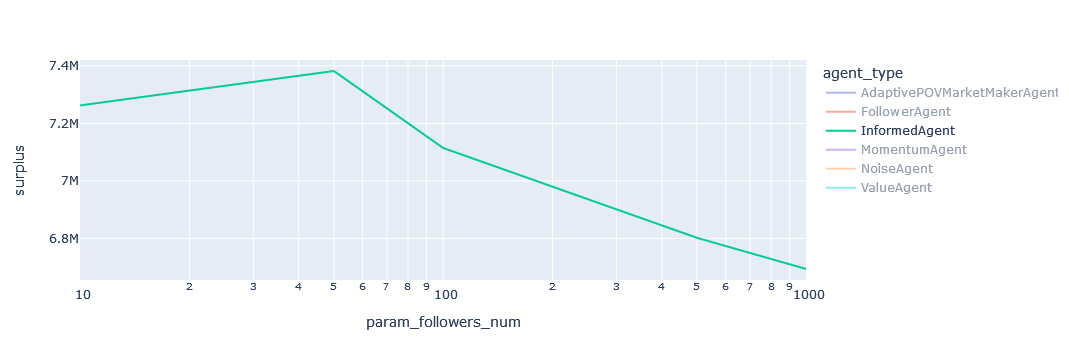
\includegraphics[scale=0.4]{informer_by_fnum.png}
\end{center}
\begin{center}
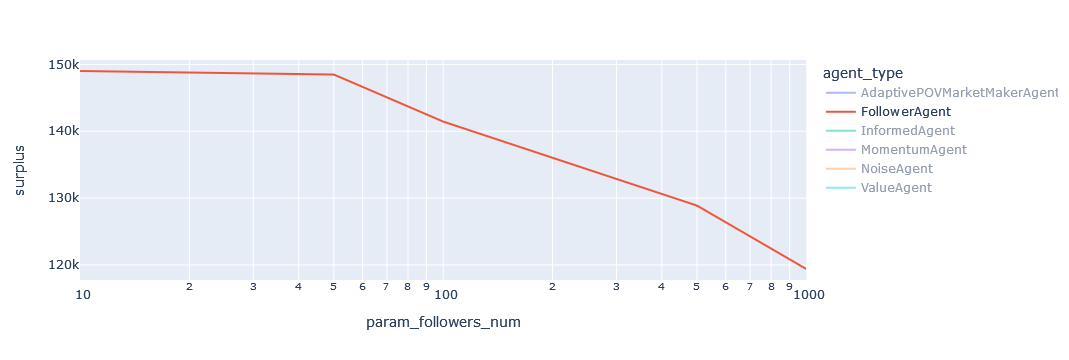
\includegraphics[scale=0.4]{follower_by_fnum.png}
\end{center}
\caption{Średnie wypłaty informatorów i obserwatorów w zależności od liczby obserwujących informatora}\label{fig:followers} 
\end{figure}
\end{center}
Prawdopodobnym uzasadnieniem tej zależności jest występowanie dla dużych grup obserwatorów małych baniek spekulacyjnych (rys. \ref{fig:ball}) - duża grupa obserwatorów równocześnie realizujących swoje zlecenia zgodnie z przyjętą bezkrytycznie rekomendacją winduje cenę ponad rzeczywistą wartość instrumentu.
\begin{center}
\begin{figure}
\begin{center}
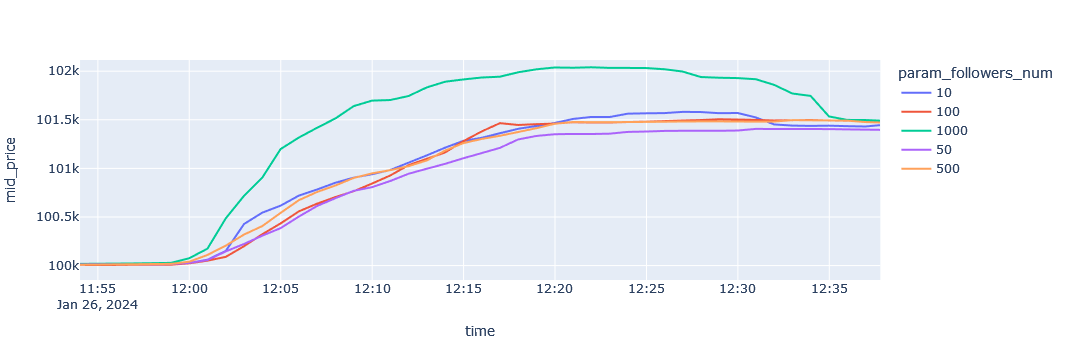
\includegraphics[scale=0.4]{ball.png}
\end{center}
\caption{Średnia cena w replikacji w zależności od liczby agentów typu \textit{FollowerAgent}}\label{fig:ball}
\end{figure}
\end{center}






% 
% wykres ceny w zależności od kapitału dla wybranej replikacji 
% wykres 